\subsection{Results}
The resonance curves we measured can be seen in Fig.\ref{fig::resonance}.
The uncertainties on the amplitudes $A$ come from two different places.
First, we can not be entirely sure that the system has reached its stationary state.
Second there is an uncertainty of $\pm 0.5 \degree$ because of the scale of the device itself.
We estimate the resulting uncertainty to $\Delta A = 2 \degree$.

The uncertainties of the angular frequencies $\omega$ come directly from the already calculated error on $C_T$ and the accuracy of the voltmeter.
Using Gaussian error propagation (\ref{eq::gauss}) on formula \ref{eq::calibration} lets us calculate $\Delta \omega$ for every measurement. 
Those uncertainties are in the magnitude of $\Delta \omega \approx 0.005 s^{-1}$, so they can be ignored (that is also why they are not shown in Fig. \ref{fig::resonance}).

\begin{figure} [ht]
	\centering
	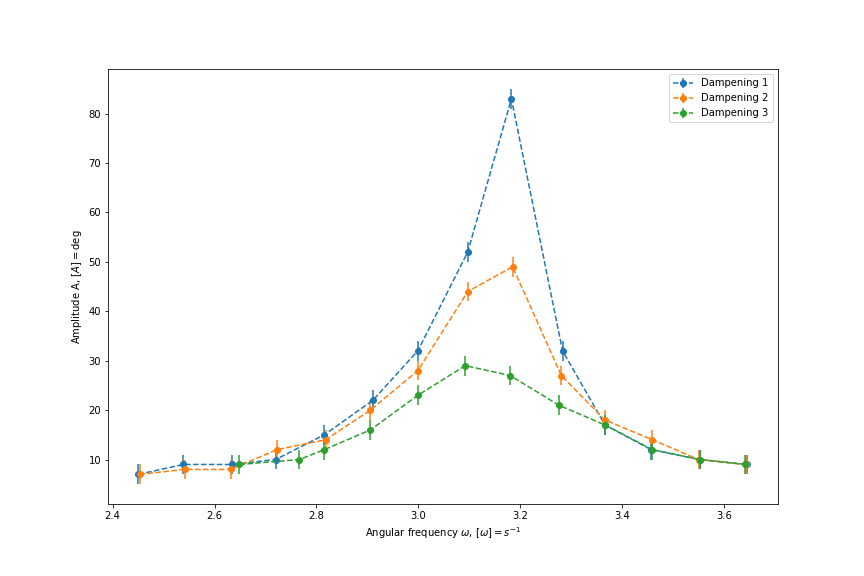
\includegraphics[width=350pt]{python/resonance.PNG}
	\caption{Measured resonance curves with errors. Errors are only shown on amplitude as they are too small to see on angular frequencies.}
	\label{fig::resonance}
\end{figure}
